\chapter{Angular mirror motion}

\section{Introduction}
For the interferometer to first achieve lock and then remain at its
linear operating point, the mirrors need to point at one another and
remain stationary with respect to this pointing. In practice, however,
the mirrors move around due to three torque inputs to each mirror: the
suspension, the actuators, and radiation pressure. Each torque
produces an angular displacement of the mirror as governed by the
mirror's torque to angle transfer function and results in either a
static or dynamic misalignment.

The dynamic misalignments arise from torque introduced through the
suspension from ground motion and through the actuators from an
unbalanced piston force. Both of these torques create an angular motion
independent of the state of the mirror's pointing. Radiation pressure
torque, however, stands apart; its effect depends on the pointing of
the mirror. A consequence is that even when all of the mirrors are
perfectly aligned at all frequencies, the simple existence of light in
the interferometer makes the arm cavities statically unstable when
high enough laser powers are used. 

This chapter discusses the causes of mirror angular displacement and
the effects of residual mirror motion on the
interferometer. Background material is provided as necessary, such as
the dynamics of torsion pendula, and the geometric eigenfunctions of
linear cavities. In all, I hope to convince the reader of the need for
an Angular Sensing and Control subsystem.





\section{The mirrors as torsion pendula}
The mirrors in LIGO are torsion pendula. They are suspended from a
single \textcolor{blue}{xx m diameter} wire that makes contact with
the bottom of the barrel of the mirror as shown in
Fig. \ref{fig:suspension}. Stand-offs glued just below the mirror's
center of mass on both sides of the barrel mark the final point of
contact of the wire with the mirror, and both ends of the wire are clamped
to the top of a suspension cage. The mirror is free to twist an angle
$\theta$ about a horizontal axis passing through its center of mass to
create motion in \emph{pitch} and about a vertical axis passing through its
center of mass to create a motion in \emph{yaw}. 

The angular equation of motion of the mirror is governed by the sum of
all torques on the mirror. First, let's consider the most simplistic scenario where
there is only a pendulum restoring torque $\tau_p=-\kappa_p \theta$,
where $\kappa_p$ is the pendulum's torsional constant. The equation of
motion is
\begin{equation}
I \ddot{\theta} + \kappa_p \theta = 0,
\end{equation}
which has a solution of $\theta(t) = \sin({\omega_0 t)}$, where
$\omega_0 = \sqrt{\kappa_p/I}$ is the resonant angular frequency and
$I$ is the mirror's moment of inertia. The pendulum torsional constant
serves to make the mirror oscillate indefinitely about its equilibrium
position upon the slightest displacement.

\begin{figure}
\begin{centering}
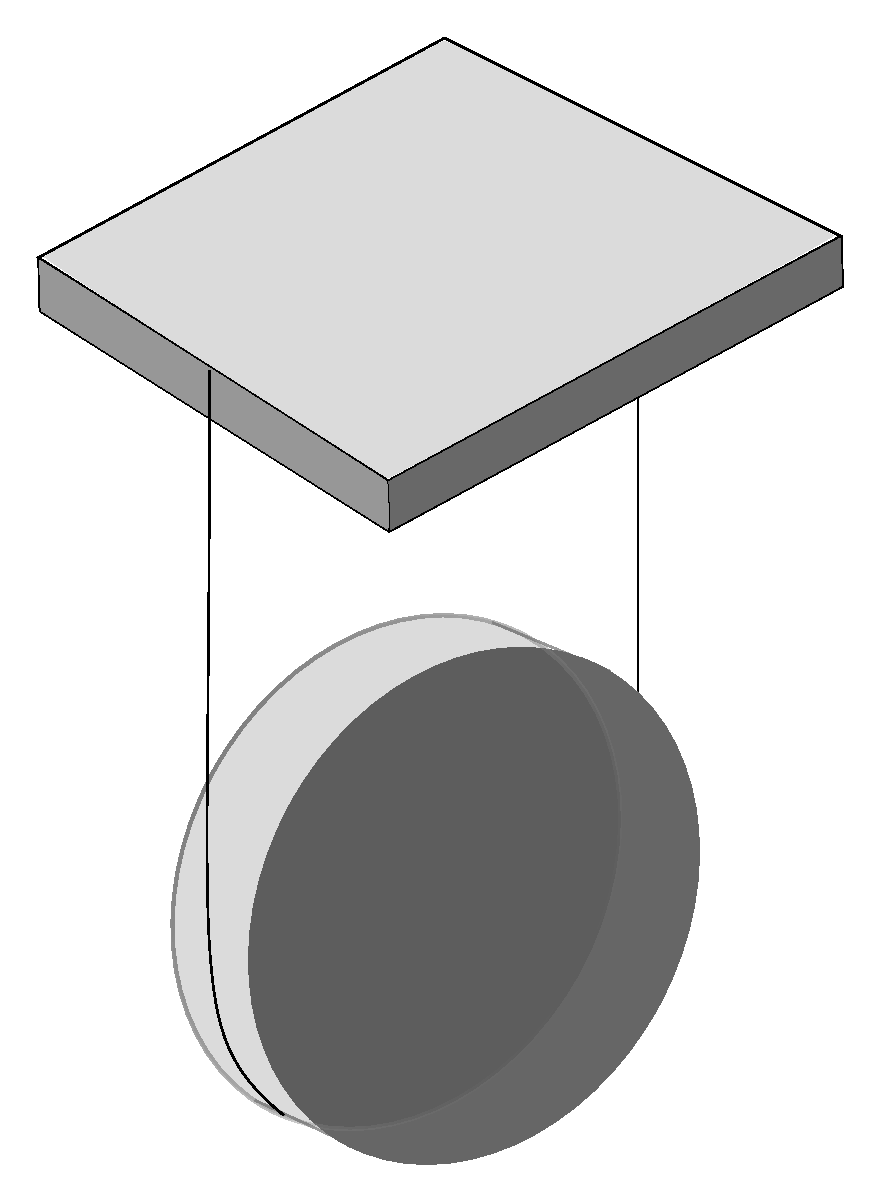
\includegraphics[width=0.3\textwidth]{/Users/kate/kate-thesis/figures/suspension.pdf}
\caption{Cartoon of a LIGO suspension. \textcolor{blue}{Improve this.}}
\label{fig:suspension}
\end{centering}
\end{figure}


\subsection{Torque to angle transfer function}
We are particularly interested in the pendulum's response to an
external torque, such as seismic noise. In order to calculate the
torque to angle transfer function, we must include an external torque
term, $\tau_{ext}$, in the equation of motion:
\begin{equation}
I \ddot{\theta} + \gamma \dot{\theta} + \kappa \theta = \tau_{ext}.
\label{eq:eqmotion}
\end{equation}
Here, we have also introduced a damping term, $\gamma$, to best model
reality. Taking the Laplace transform to convert from the time domain
to the frequency domain, we have:
\begin{equation}
I s^2 \Theta + \gamma s \Theta + \kappa \Theta = \tau_{ext}
\end{equation}
where $s$ is a complex parameter. We are only interested in examining
the transfer function for a pure sine wave excitation, $e^{i\omega
  t}$, so we substitute $s=i\omega$ to get
\begin{equation}
\mathrm{TF} := \frac{\Theta}{\tau_{ext}} = \frac{1}{I s^2 + \gamma s +
  \kappa} = \frac{1/I}{\omega_0^2  - \omega^2 + i \gamma \omega / I}
\label{eq:TF}
\end{equation}
which has poles at 
\begin{equation}
s = s_\pm = \frac{-\gamma \pm \sqrt{\gamma^2 - 4 I \kappa}}{2 I}.
\label{eq:TFpoles}
\end{equation}
The resonant frequency of this system can be computed by finding the
$\omega$ at which the amplitude of the transfer function, $[I^2
[\omega^2 - \omega_0^2]^2 + \gamma^2 \omega^2]^{-1/2}$, is maximized:
\begin{equation}
\omega_{res} = \sqrt{\omega_0^2 - \frac{\gamma^2}{2I^2}}.
\end{equation}
We see that damping serves to reduce the resonant frequency.

A quantity used more often than $\gamma$ for describing the losses of
a system with a real resonance is the quality factor,
$Q~:=~\omega_{res}/\mathrm{FWHM}$, where FWHM is that computed for the
amplitude squared of the transfer function. When the losses are small,
$\omega_{res} \approx \omega_0$ and FWHM $\approx \gamma/I$ (see
Feynman 23-4). The quality factor is then well approximated by $Q =
\sqrt{\kappa I}/\gamma$. The transfer function written in terms of $Q$
is
\begin{equation}
\mathrm{TF} = \frac{1/I}{\omega_0^2  - \omega^2 + i \omega \omega_0 / Q}.
\label{eq:TFpendulum}
\end{equation}
Figure \ref{fig:pendTF} shows this torque to angle transfer function
(for pitch) using the parameters of a LIGO core optic. For external
torques applied to the mirror above its resonant frequency, the mirror
acts like a free mass, one that is not held in place by suspension
wires nor subject to damping. For torques applied to the mirror below
its resonant frequency, the mirror's angle is determined by the
inverse of the torsional constant.

\begin{figure}
\begin{centering}
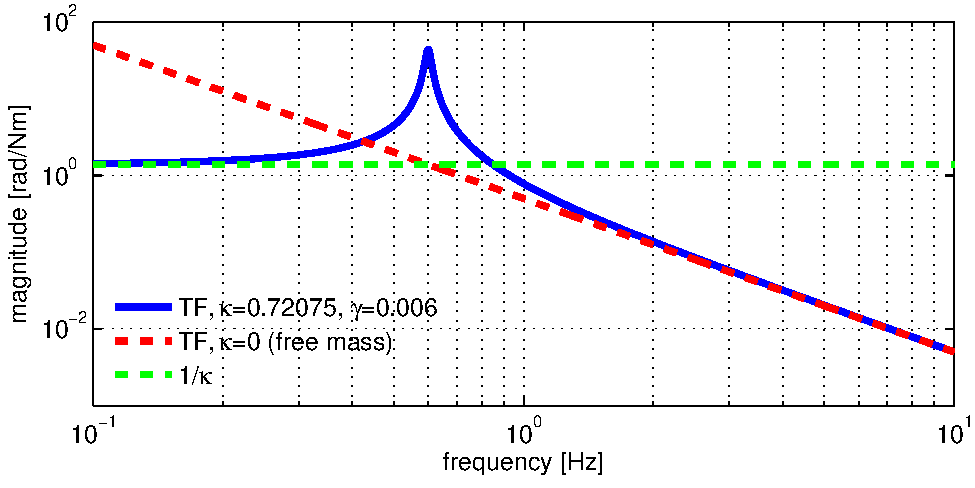
\includegraphics[width=0.7\textwidth]{figures/pendTF.pdf}
\caption{Torque to pitch transfer function of a LIGO core optic
  (blue). The optic acts like a free mass at high frequencies (green)
  and the DC magnitude of the transfer function is determined by the
  inverse torsional constant (red). A damping constant $\gamma =
  0.006$ ($Q=32$) was selected for pictorial reasons only. The
  resonant frequency of LIGO core optics in yaw is 0.5~Hz.}
\label{fig:pendTF}
\end{centering}
\end{figure}




\section{Seismic noise torque}
Ground motion couples through both the seismic isolation table and the
suspension. The torque it induces on the mirror creates pitch or yaw
motion according to the torque to angle transfer function,
Eq. \ref{eq:TFpendulum}. An example of the motion of the core test
masses during a time of relatively quiet seismic noise at LLO is shown
in Fig. \ref{fig:seismicMirror}.

At all times, whether the interferometer is locked or not, all
suspended optics are velocity damped by the OSEM actuators. In
addition, the 6 core optics are velocity damped by optical levers as
well. The spectra in the figure are taken in the presence of this AC
damping--it is, after all, the motion that will need to be controlled
interferometrically.

% Take a model of the optical lever open loop gains and a spectrum of
% optical lever error signal at a time when the interferometer is
% unlocked, but optical levers are on to calculate the background mirror
% motion due to seismic noise. Show the effect at a select few different
% times of day, probably for just one mirror. Write this section once I
% see what I have to present.

\begin{figure}
\begin{centering}
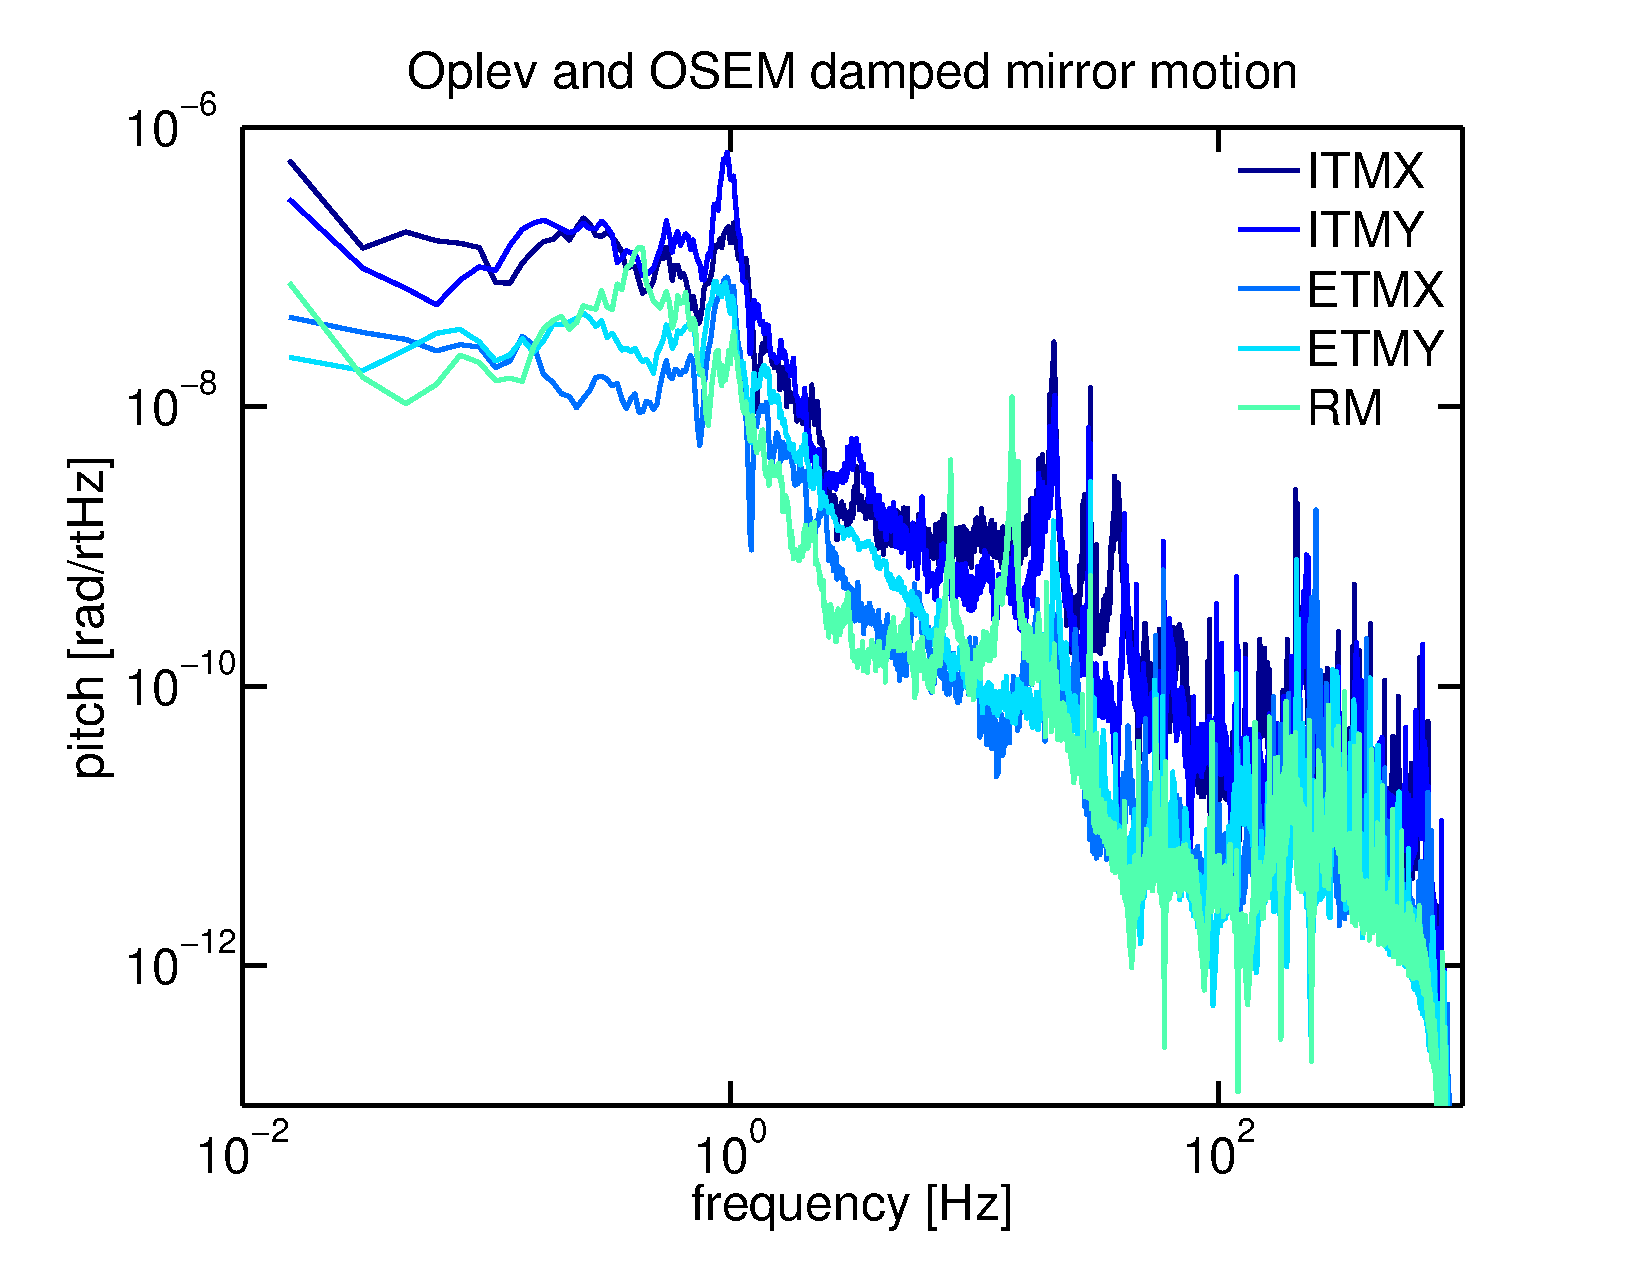
\includegraphics[width=0.7\columnwidth]{figures/ifodark_mirrormotion.pdf}
\caption{Typical angular motion of the core suspended mirrors in the
  absence of interferometric control. Velocity damping provided by the
  OSEMs and the optical levers is present. Above about 30 Hz, the plot
  does not represent real motion; the spectrum is limited by sensor
  (optical lever) noise. \textcolor{blue}{Show the quadrature sum of
    angular motion due to the three sources discussed in this
    section.}}
\label{fig:seismicMirror}
\end{centering}
\end{figure}


\section{Actuation noise torque}
Length control couples to angle when the two are not perfectly
diagonalized.  Each mirror is equipped with four optical sensor and
electro-magnetic (OSEM) actuators for providing control to the
mirror. Magnets arranged to form the four corners of a square are
glued on the mirror's back surface, and the OSEM units envelop
them. Length control of the cavities sends current of the same
magnitude through each coil on a given mirror to provide a piston
force for changing the mirror's position. However, small misbalances
in inductor and magnetic strength result in a torque actuation in
addition to a position actuation. This length to angle coupling,
$\alpha$, is on the order of 1\%.

A typical length control signal provides a force with such and such a
spectrum in units of m/rtHz, which means the angular motion induced by
L2A is as shown in Fig. \ref{}.

\begin{figure}
\begin{centering}
%\includegraphics[width=0.6\columnwidth]{figures/}
\caption{Angular motion induced by a 1\% coupling of length actuation to angle.}
\label{fig:}
\end{centering}
\end{figure}




\section{Radiation pressure torque}
Radiation pressure creates a torque when the beam impinges the mirror
off-center. The force on the mirror due to radiation pressure is
derived from the change in momentum of a photon upon reflection off
the mirror and results in:
\begin{equation}
F_{rp} = \frac{2 P} {c}.
\end{equation}
$P$ is the power of the light reflected by the mirror and $c$ is the
speed of light. Assuming the beam of photons strikes the mirror
perpendicular to its surface, the torque exerted on a mirror due to
radiation pressure is
\begin{equation}
\tau_{rp} = \frac{2 P x} {c}
\label{eq:tau_rp}
\end{equation}
where $x$ is the distance of the beam from the mirror's center of
mass. 

For LIGO we must consider the effect of $\tau_{rp}$ on mirrors that
form a linear cavity. As we show in the following subsection, the beam
positions are coupled and dependent on the angles of the mirrors. The
radiation pressure torques are likewise coupled to both mirrors. They
create two orthogonal and power-dependent opto-mechanical modes
through modification of the pendulum torque to angle transfer
function, Eq. \ref{eq:TFpendulum}. In all, radiation pressure shapes
the angular dynamics of the mirrors in LIGO and plays an important
role in the design of an angular control system.


\subsection{Tilt eigenmodes of a Fabry-Perot cavity}
For a Fabry-Perot cavity as is used in the arms of the LIGO
interferometer, the positions of the beams on the mirrors $x_i$ are
dependent on the angles of the mirrors $\theta_i$ according to the
cavity's geometry:
\begin{equation}
\left\llbracket \begin{array}{c}
x_1\\
x_2 \end{array} \right\rrbracket = \frac{L}{1-g_1 g_2}
\left\llbracket \begin{array}{cc}
g_2 & 1\\
1 & g_1\end{array} \right\rrbracket
\left\llbracket \begin{array}{c}
\theta_1\\
\theta_2 \end{array} \right\rrbracket .
\label{eq:x}
\end{equation}
The g-factor is defined as $g_i=1-R_i/L$ where $R$ is the radius of
curvature of the mirror and $L$ is the length of the cavity. 

It is informative to diagonalize this matrix, $\mathbf{A}
=\left\llbracket \begin{array}{cc}g_2 & 1\\1 & g_1\end{array}
\right\rrbracket $, and see what sets of mirror tilts and beam
positions are independent from one another. Its eigenvalues are
\begin{align}
\lambda_1 &= \frac{g_1 + g_2 + \sqrt{(g_1 - g_2)^2 + 4}}{2} \\
\lambda_2 &= \frac{g_1 + g_2 - \sqrt{(g_1 - g_2)^2 + 4}}{2} \label{eq:eigenvalues}
\end{align}
and its eigenvectors are
\begin{align}
\vec{v}_1 &= \left\llbracket \begin{array}{c} 
1 \\
\frac{g_1 - g_2 + \sqrt{(g_1 - g_2)^2 + 4}} {2} \end{array} \right\rrbracket\\
\vec{v}_2 &= \left\llbracket \begin{array}{c}
\frac{ -g_1 + g_2 - \sqrt{(g_1 - g_2)^2 + 4}}{2} \label{eq:eigenvectors}\\
1 \end{array} \right\rrbracket .
\end{align}
Therefore, the matrix 
\begin{equation}
\mathbf{P} = \left\llbracket \begin{array}{cc} 
\vec{v}_1 & \vec{v}_2 \end{array} \right\rrbracket =
\left\llbracket \begin{array}{cc}
 1 & \frac{-g_1 + g_2 - \sqrt{(g_1 - g_2)^2 + 4}} {2}\\
 \frac{g_1 - g_2 + \sqrt{(g_1 - g_2)^2 + 4}} {2} & 1\end{array} \right\rrbracket
\end{equation}
diagonalizes $\mathbf{A}$ such that 
\begin{equation}
\mathbf{P^{-1}AP} = \left\llbracket \begin{array}{cc} 
\lambda_1 & 0 \\
0 & \lambda_2 \end{array} \right\rrbracket = \left\llbracket \begin{array}{cc}
 \frac{g_1 + g_2 + \sqrt{(g_1 - g_2)^2 + 4}}{2}  & 0\\
 0 & \frac{g_1 + g_2 - \sqrt{(g_1 - g_2)^2 + 4}}{2}\end{array} \right\rrbracket .
\end{equation}

These eigenvectors $\vec{v}_1$ and $\vec{v}_2$ form the orthogonal
bases of mirror tilts in which we will describe each of the arm
cavities for the remainder of this dissertation. In particular, since
$\mathbf{A} \vec{v} = \lambda \vec{v}$, the beam displacements are
proportional to the mirror tilts when the tilts are described by one
of these two eigenvectors. Figure \ref{fig:ss} illustrates a cavity in
each of these two \emph{eigenmodes} when using the LIGO cavity parameters
as outlined in Table \ref{table:cav_geometric}. The derivation of the
dependence of cavity displacement $a$ and cavity tilt $\alpha$ on
mirror angles is in Appendix xx.


\begin{figure}
\begin{centering}
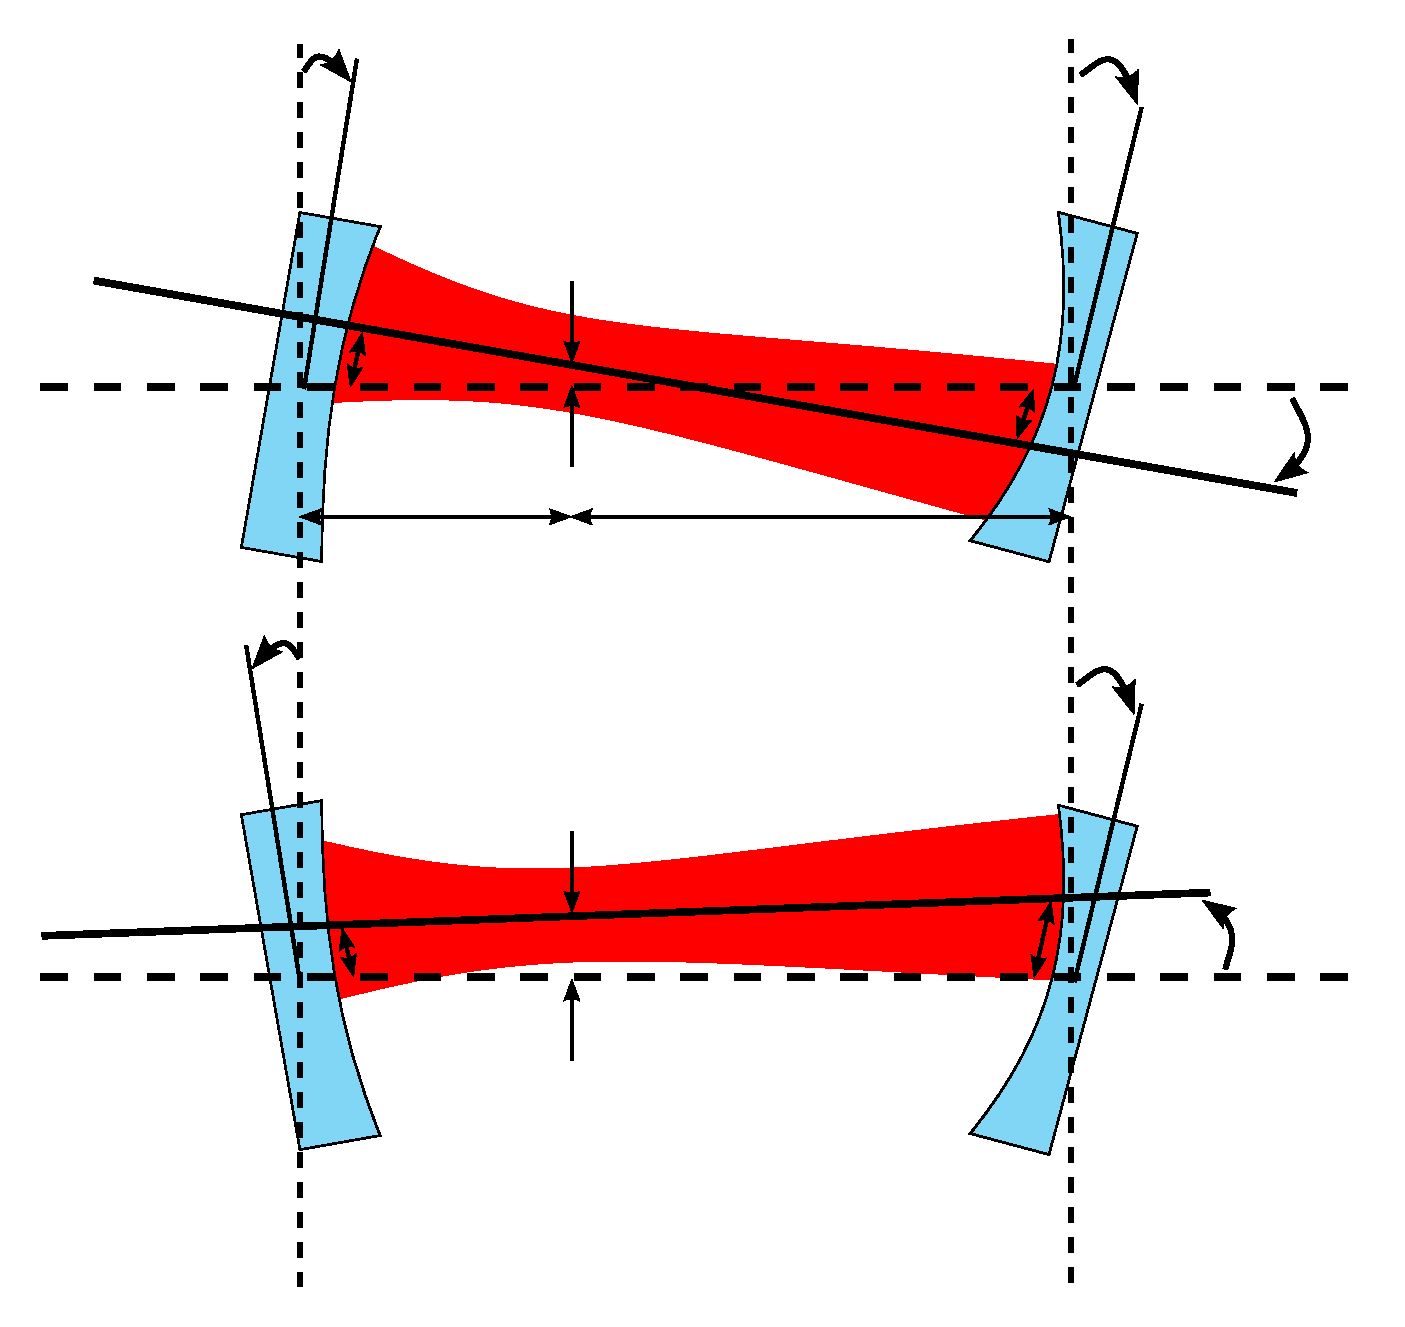
\includegraphics[width=0.6\columnwidth]{figures/eigenmodes.pdf}
\caption{Illustration of the orthogonal modes of cavity tilt. The upper diagram shows tilts given
  by eigenvector $\vec{v}_2$ and the lower diagram shows $\vec{v}_1$.} 
\label{fig:ss}
\end{centering}
\end{figure}

\begin{table}
\centering
\caption{Geometric parameters of the LIGO arm cavity
  eigenmodes. $x_i$ are the beam locations on the mirrors relative
  to center, $a$ is the cavity axis displacement at the waist, and
  $\alpha$ is the cavity axis angle with respect to a line joining the
centers of the mirrors. Differences between LLO and LHO arise from the
mirrors having different radii of curvature at the two sites.}
\begin{tabular}{l l l l l}
& LLO & LLO & LHO & LHO \\
cavity parameter & $\vec{v}_1$ mode & $\vec{v}_2$ mode & $\vec{v}_1$ mode & $\vec{v}_2$ mode \\
\hline\hline
$|x_1|$ [mm/urad]  & 9.88 & 2.44 & 8.20 & 2.51\\
$|x_2|$ [mm/urad] & 10.84 & 2.22 & 9.35 & 2.20\\
$|a|$ [mm/urad] & 10.17 & 1.01 & 8.48 & 1.34 \\
$|\alpha|$ [urad/urad] & 0.24 & 1.17 & 0.29 & 1.18 \\
\hline
\end{tabular}
\label{table:cav_geometric}
\end{table}



\subsection{Soft and hard modes}
We have seen that mirror torques due to radiation pressure are a
function of beam positions (Eq. \ref{eq:tau_rp}) and that beam
positions are a function of mirror angles (Eq. \ref{eq:x}). We are now
ready to combine these two observations to define radiation pressure
torque as a function of mirror angle:
\begin{equation}
\left\llbracket \begin{array}{c}
\tau_{rp,1}\\
\tau_{rp,2} \end{array} \right\rrbracket = \frac{2 P L}{c (1-g_1 g_2)}
\left\llbracket \begin{array}{cc}
g_2 & 1\\
1 & g_1\end{array} \right\rrbracket
\left\llbracket \begin{array}{c}
\theta_1\\
\theta_2 \end{array} \right\rrbracket.
\end{equation}
This is more succinctly expressed as
\begin{equation}
\vec{\tau}_{rp} = -\mathbf{K_{rp}} \vec{\theta},
\end{equation}
where $\mathbf{K_{rp}}$ is called the \emph{torsional stiffness matrix}. 

We arrive at the purpose of this section--to evaluate how radiation
pressure affects the suspended mirror's motion. In order to examine
its effect, we will work in the basis of the diagonalized
$\mathbf{K_{rp}}$, using the eigenvectors $\vec{v}_1$ and $\vec{v}_2$
as two different cases of mirror tilts. The total torque on each
mirror for each of these two cases ($i=1,2$) is the sum of the
restoring torque of the pendulum and the radiation pressure torque:
\begin{align}
\vec{\tau}_{tot_i} = \vec{\tau}_{rp} + \vec{\tau}_{p} &= -[\kappa_{rp_i} + \kappa_p] \vec{v}_i \\
&= -\left[- \frac{2 P L}{c (1-g_1 g_2)} \lambda_i + \kappa_{p}\right] \vec{v}_i \\
&:= -\kappa_{tot_i} \vec{v}_i
\label{eq:torque_tot}
\end{align}
with $\lambda_i$ and $\vec{v}_i$ defined by Eqs. (\ref{eq:eigenvalues}) and (\ref{eq:eigenvectors}).


Here we make an observation of great significance for the rest of the
paper. While the new torsional constant, $\kappa_{tot_i}$, is
positive, the torque is restorative and the mirror will 
return to its equilibrium position. However, as soon as $\kappa_{tot_i}$
becomes negative, the system is unstable as the mirror will be pushed
yet further away from equilibrium. And of course, when $\kappa_{tot_i}=0$,
$\tau_{tot_i}=0$. Explicitly, our stability criteria are 
\begin{align}
\mbox{stable: } &\frac{2 P L \lambda_i}{c (1-g_1 g_2)} < \kappa_p \\
\mbox{unstable: } &\frac{2 P L \lambda_i}{c (1-g_1 g_2)} > \kappa_p.
\label{eq:stability}
\end{align}

We now turn to examine this stability criteria for the specific case
of LIGO's arm cavities. First, in order for a Gaussian beam to fit
properly between two mirrors and thus form a resonant cavity, the
g-factors are restricted to $0 < g_1g_2 < 1$. Therefore, the sign of
the left-hand side of Eq. \ref{eq:stability} is determined solely by
that of $\lambda$, and it can be shown from the g-parameter
restriction that $\lambda_1$ is always positive and $\lambda_2$ is
always negative. Since $\kappa_p > 0$, the mode described by
$\vec{v}_1$ will be either stable or unstable, and the mode described
by $\vec{v}_2$ will always be stable. Namely, as power $P$ increases,
$\kappa_{tot_1}$ decreases, creating a softer spring, but
$\kappa_{tot_2}$ increases, creating a stiffer spring. Thus arise the
terms \emph{soft} and \emph{hard} to describe the two
eigenmodes. 

To see how radiation pressure modifies the torque to angle transfer
function of the pendula, $\kappa_{tot}$ is used in
Eq. \ref{eq:TFpendulum} instead of just $\kappa_{p}$. The effect is that $\omega_0$ is now
not only a function of $\kappa_p$, but also of $\kappa_{rp}$:
\begin{align}
\mathrm{soft: } \omega_0 &= \sqrt{\frac{- \frac{2 P L}{c (1-g_1 g_2)} \frac{g_1 + g_2 + \sqrt{(g_1 - g_2)^2 +
      4}}{2} + \kappa_p}{I}} \\
\mathrm{hard: } \omega_0 &= \sqrt{\frac{- \frac{2 P L}{c (1-g_1 g_2)} \frac{g_1 + g_2 - \sqrt{(g_1 - g_2)^2 +
      4}}{2} + \kappa_p}{I}}
\end{align}
Figure~\ref{fig:kf_hardsoft} shows $\kappa_{tot_i}$ for a LIGO arm
cavity as a function of circulating power and Table \ref{table:k_tot}
highlights the specific numbers for Initial and Enhanced LIGO
powers. The corresponding hard and soft transfer functions are plotted
in Fig. \ref{fig:optomechhardsoft}.


\begin{figure}
\begin{centering}
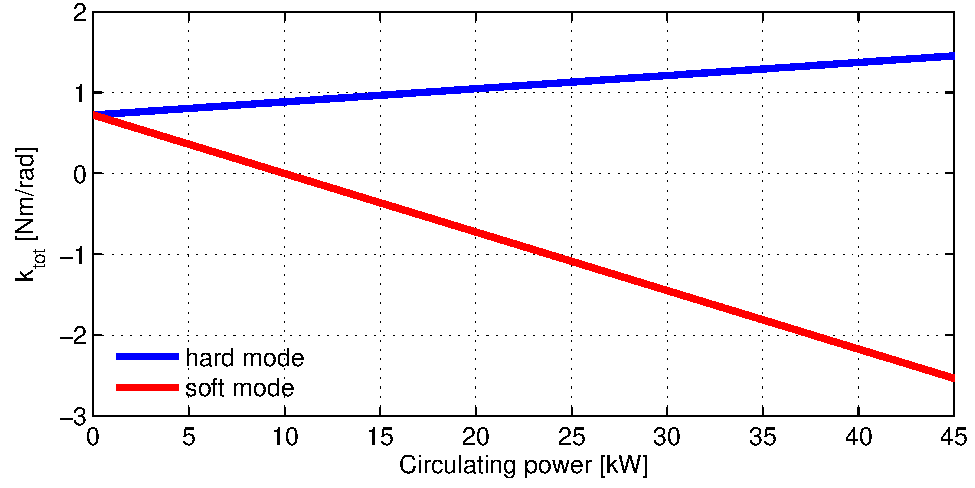
\includegraphics[width=0.8\textwidth]{figures/khardsoftLLO.pdf}
\caption{Torsional spring constants (pitch) of an optically coupled
  cavity for LLO parameters. The soft mode is unstable when the spring
  constant is negative.}
\label{fig:kf_hardsoft}
\end{centering}
\end{figure}


\begin{table}
\centering
\caption{Torsional constants (pitch) for the soft and hard modes of a typical
  Initial LIGO power and the highest of Enhanced LIGO powers. The soft
mode in Enhanced LIGO is unstable.}
\begin{tabular}{l l l l l}
 & $P_{circ}$ & $\kappa_{p}$ & $\kappa_{tot_1}$, soft &
 $\kappa_{tot_2}$, hard \\
 & (kW) & (Nm/rad) & (Nm/rad) & (Nm/rad) \\
\hline\hline
iLIGO & 9 & 0.721 & 0.0734 & 0.867 \\
eLIGO & 40 & 0.721 & -2.18 & 1.38 \\
\hline
\end{tabular}
\label{table:k_tot}
\end{table}



\begin{figure}
\begin{centering}
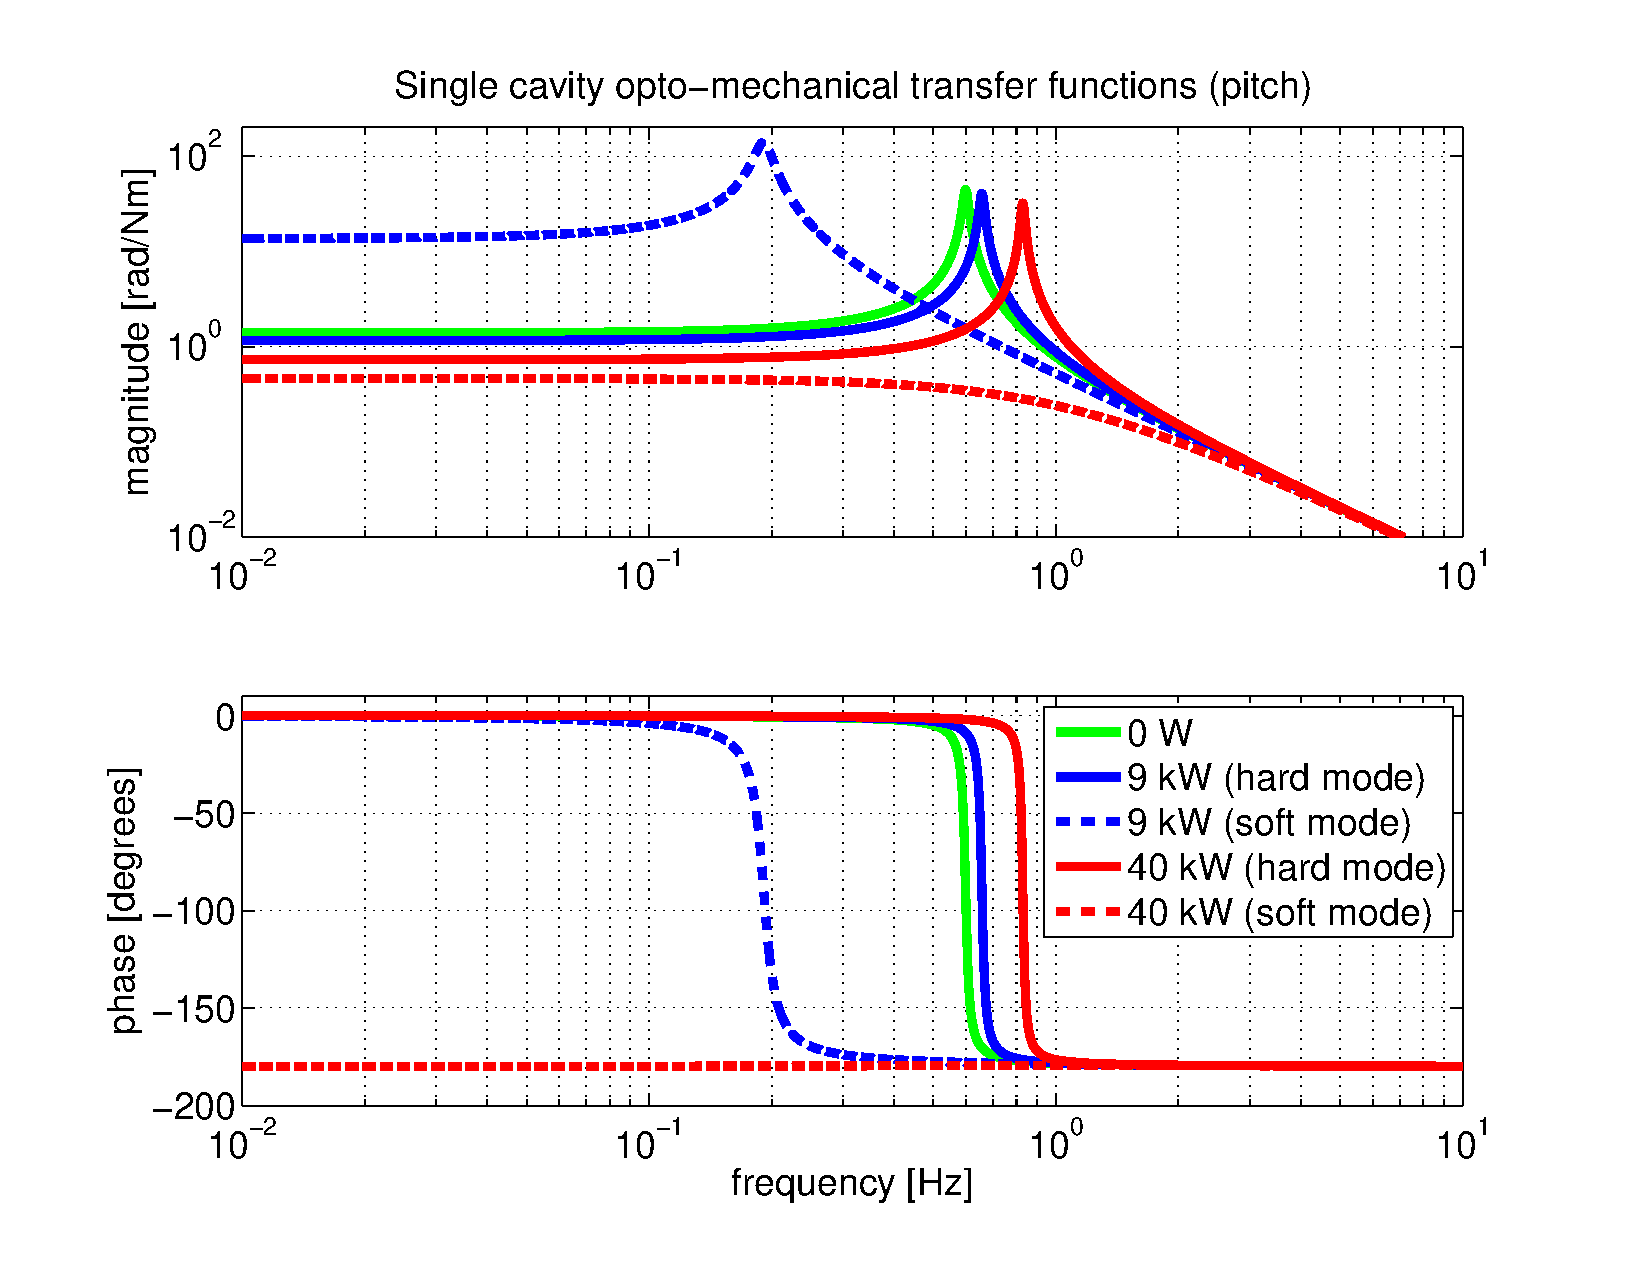
\includegraphics[width=0.8\textwidth]{figures/iLIGOeLIGOhardsoftmodes.pdf}
\caption{Single cavity opto-mechanical transfer function for
  pitch. The resonant frequency increases with power for the hard
  mode, but decreases for the soft mode, eventually becoming
  imaginary. $P_{circ} = 9$ kW (5.25 W input) was a typical operating power for
  Initial LIGO and $P_{circ} = 40$ kW (23.5 W input) is the highest of powers reached
for Enhanced LIGO.}
\label{fig:optomechhardsoft}
\end{centering}
\end{figure}


\subsection{Stability}
Let's re-examine the stability criteria, but from the transfer
function perspective. The poles $s_\pm$ of the transfer function
indicate whether a system will respond to an excitation in a
sinusoidal and/or exponential matter since the inverse Laplace
transform of the transfer function is the impulse response. As long as
the poles are negative real or imaginary, the angular motion will
decay or be sinusoidal. However, if a pole is in the right half of the
s-plane, the system's motion will experience exponential growth.

Referring to the equation for the poles, Eq. \ref{eq:TFpoles}, we can
make a table of conditions on $\kappa$ for $s_\pm$ to be in a
particular half of the s-plane. First, we notice that $s_-$ will
always be in the left half of the plane or along the imaginary axis
and that $s_+$ is the potentially problematic pole. All possibilities
for the pole in question are enumerated in Table \ref{table:s_0} and
demonstrate that as is shown in the previous subsection, stability is
determined by the sign of $\kappa$. Figure \ref{fig:pendTF_k} shows
how the pole location changes as a function of $\kappa$.


\begin{table}
\centering
\caption{Conditions on torsional constant $\kappa$ for determining
 system stability.}
\begin{tabular}{l l l}
$\kappa$ condition & pole $s_+$ & impulse response \\
\hline\hline
$\kappa < 0$ & real positive & statically unstable\\
$\kappa = 0$ & zero & \\
$0 < \kappa < \gamma^2/4I $ & real negative & stable decay \\
$\kappa > \gamma^2/4I$ & real negative, and imaginary & stable,
oscillatory \\
\hline
\end{tabular}
\label{table:s_0}
\end{table}

\begin{figure}
\begin{centering}
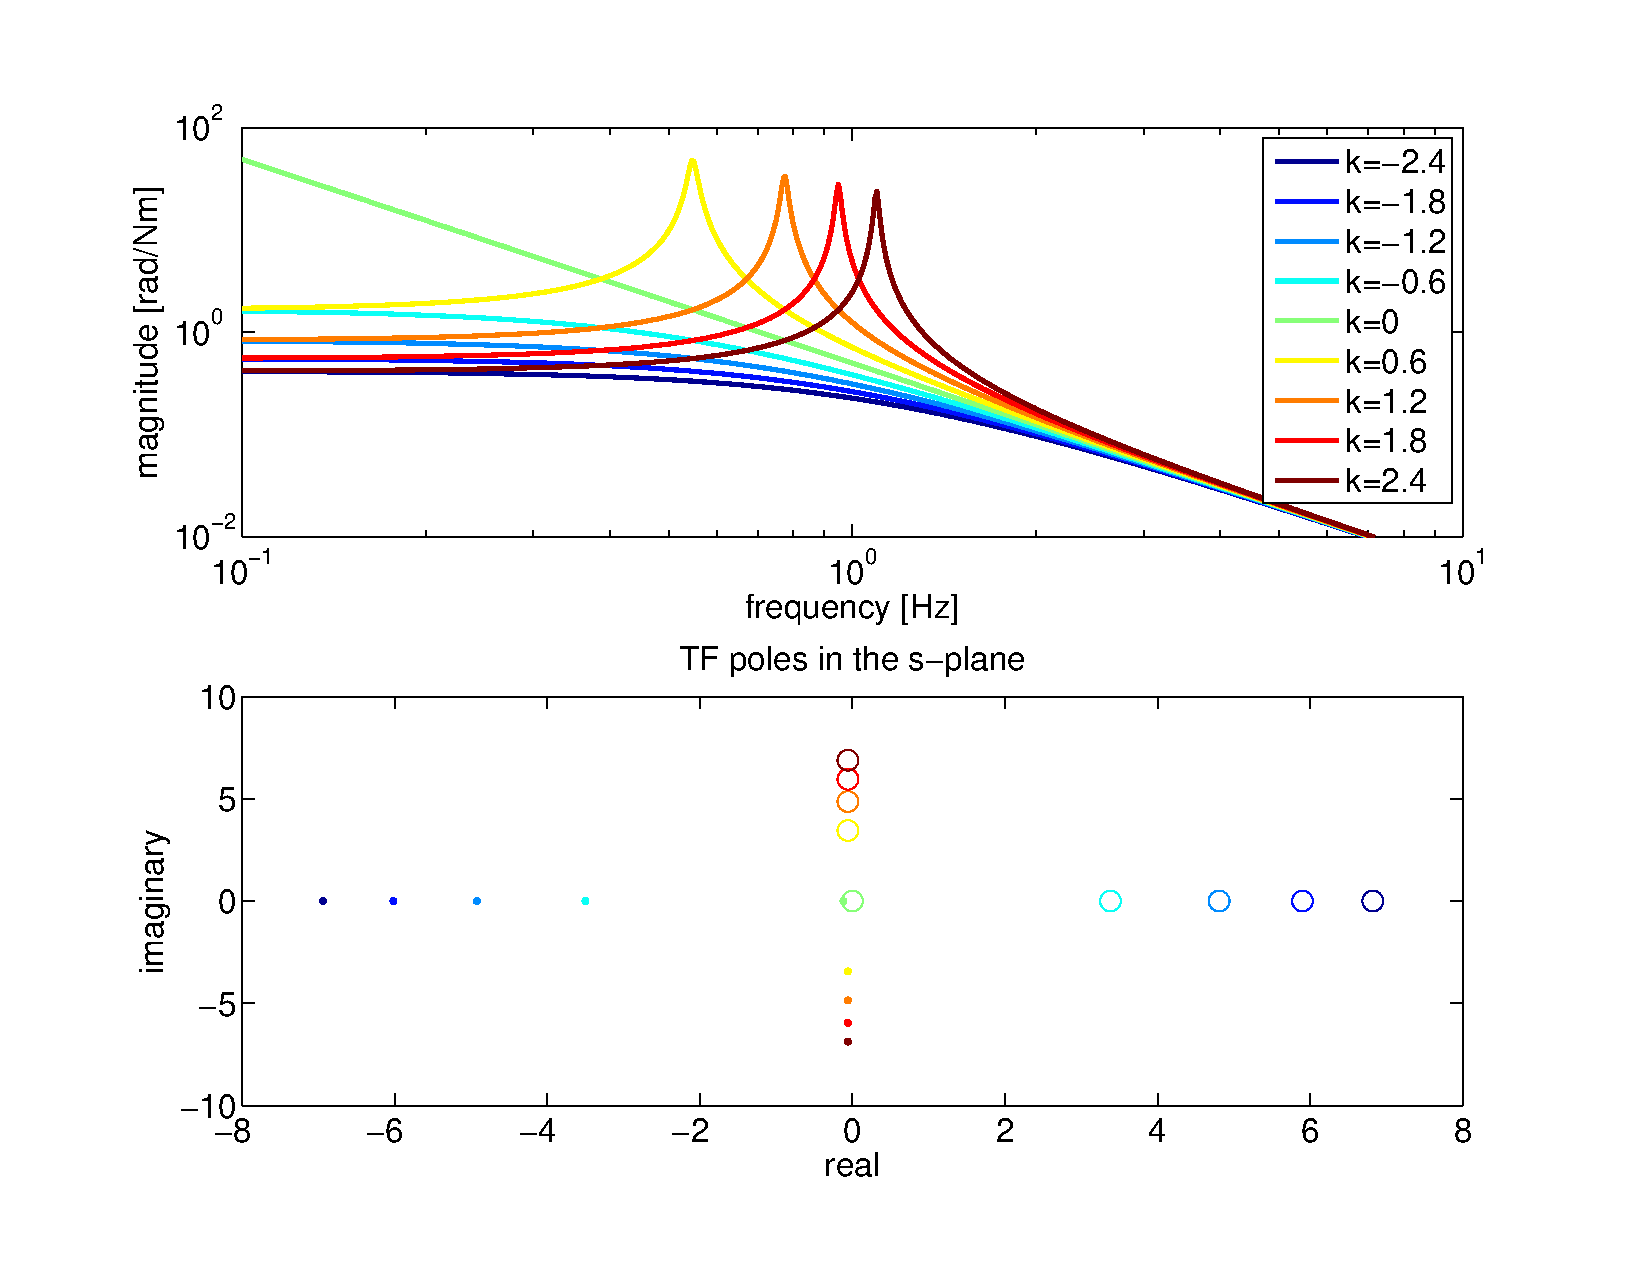
\includegraphics[width=1.0\textwidth]{figures/pendTF_k.pdf}
\caption{Torque to pitch transfer function (upper plot) and poles
  (lower plot) as a function of torsional constant for a fixed damping
  coefficient of $\gamma^2/4I = 1.77 \times 10^{-4}$. Circles show
  $s_+$ and dots show $s_-$. Poles in the right half of the s-plane
  indicate the system is unstable. This range of $\kappa$ represents
  the torsional constants experienced while powering up Enhanced
  LIGO.}
\label{fig:pendTF_k}
\end{centering}
\end{figure}









\section{How much suppression is necessary?}
The requirements for the amount of angular suppression arise from the
effect of residual angular motion on the interferometer. Power
fluctuations in the interferometer, for example, put sidebands on all
lines in the DARM spectra at the frequency of the fluctuations,
creating broadband up-conversion. Misalignment can create a contrast
defect, a difference in the amount of power in one arm compared to the
other.





\section{Appendix xx--misaligned cavity axis}
Here I provide the geometric argument that shows how to calculate the
tilt $a$ and displacement $\alpha$ of a cavity as a function of mirror
misalignment. Cavity tilt is defined by the angle formed between
the line that connects the two beam spots (as given by Eq. \ref{eq:x}) and the line joining the
centers of the mirrors. Cavity displacement uses the same two lines,
yet is defined by the distance between them at the location of the
waist of the resonant spatial mode. Based on pure geometry, the cavity
displacement and tilt are:
\begin{equation}
\left\llbracket \begin{array}{c}
a \\
\alpha \end{array} \right\rrbracket = \frac{1}{L}
\left\llbracket \begin{array}{cc}
z_2 & z_1\\
-1 & 1\end{array} \right\rrbracket
\left\llbracket \begin{array}{c}
x_1\\
x_2 \end{array} \right\rrbracket
\label{eq:cavitydisptilt}
\end{equation}
where $z_i$ is the distance to the waist from mirror $i$ calculated as:
\begin{eqnarray}
z_1 &=& \frac{g_2 (1-g_1) L}{g_1+g_2 - 2 g_1g_2} \\
z_2 &=& L - z_1.
\end{eqnarray}

Clearly, we can combine Eqs. (\ref{eq:x}) and
(\ref{eq:cavitydisptilt}) to arrive at an equation directly relating
mirror tilt to cavity displacement and tilt: 
\begin{equation}
\left\llbracket \begin{array}{c}
a \\
\alpha \end{array} \right\rrbracket = \frac{1}{1-g_1g_2}
\left\llbracket \begin{array}{cc}
g_2z_2 + z_1 & z_2 + g_1z_1\\
-g_2 + 1 & -1 + g_2\end{array} \right\rrbracket
\left\llbracket \begin{array}{c}
\theta_1\\
\theta_2 \end{array} \right\rrbracket.
\label{eq:cavitydisptilt_mirrorangle}
\end{equation}